%!TEX TS-program = xelatex
\documentclass[]{friggeri-cv}
\usepackage{afterpage}
\usepackage{hyperref}
\usepackage{color}
\usepackage{xcolor}
\hypersetup{
    pdftitle={},
    pdfauthor={},
    pdfsubject={},
    pdfkeywords={},
    colorlinks=false,       % no lik border color
   allbordercolors=white    % white border color for all
}
\addbibresource{bibliography.bib}
\RequirePackage{xcolor}
\definecolor{pblue}{HTML}{0395DE}

\begin{document}
\header{Nguyen Van}{ Manh}
      {Computer Engineer}
      
% Fake text to add separator      
\fcolorbox{white}{gray}{\parbox{\dimexpr\textwidth-2\fboxsep-2\fboxrule}{%
.....
}}

% In the aside, each new line forces a line break
\begin{aside}
  \section{Address}
    273/22 To Hien Thanh,
    District 10, Ho Chi Minh, Viet Nam
    ~
  \section{Tel \& Skype}
    (+39) 902 686 220
    manhnguyen510
    ~
  \section{Mail}
    \href{mailto:manhnguyen510@gmail.com}{\textbf{manhnguyen510@}\\gmail.com}
    ~
  \section{Web \& Git}
    \href{https://github.com/vmnguyen}{github.com/vmnguyen}
    ~
  \section{Programming}
    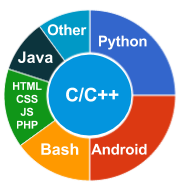
\includegraphics[scale=0.62]{img/programming.png}
    ~
  \section{OS Preference}
    \textbf{GNU/Linux}
\includegraphics[scale=0.40]{img/4stars.png}
    \textbf{Windows}
\includegraphics[scale=0.40]{img/3stars.png}
    ~
  \section{Personal Skills}
    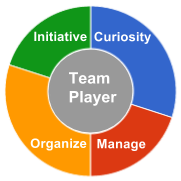
\includegraphics[scale=0.62]{img/personal.png}
    ~
  \section{Languages}
    \textbf{Vietnamese}
\includegraphics[scale=0.40]{img/5stars.png}
    \textbf{English}
\includegraphics[scale=0.40]{img/3stars.png}
\end{aside}
\section{Experience}
\begin{entrylist}
    \entry
    {20/06 - 30/09}
    {Internship}
    {ISB-Vietnam Company Limited}
    {Management and migration of servers. Development of web templates and interfaces. Management of SQL databases.}
\end{entrylist}

\section{Education}
\begin{entrylist}
  \entry
    {2013 - 2018}
    {Bachelor's Degree in Computer Engineering}
    {Università di Pisa, Italy}
    {Main subjects: Matematics and Physics, Programming, Operational Research, Telecommunication Systems, Digital and Analogical Electronics.\\
    \emph{Title of the Thesis: "Development, Management and Migrations of web contents and applications".}\\
    \emph{Thesis activity carried out during an internship period at Atitlan Engineering SRL.}\\}
\end{entrylist}

\section{Certifications}
\begin{entrylist}
  \entry
    {10/2016}
    {Machine Learning}
    {Coursera. E-learning}
    {\emph{Stanford University}}
\end{entrylist}


%%% This piece of code has been commented by Karol Kozioł due to biblatex errors. 
% 
%\printbibsection{article}{article in peer-reviewed journal}
%\begin{refsection}
%  \nocite{*}
%  \printbibliography[sorting=chronological, type=inproceedings, title={international peer-reviewed conferences/proceedings}, notkeyword={france}, heading=subbibliography]
%\end{refsection}
%\begin{refsection}
%  \nocite{*}
%  \printbibliography[sorting=chronological, type=inproceedings, title={local peer-reviewed conferences/proceedings}, keyword={france}, heading=subbibliography]
%\end{refsection}
%\printbibsection{misc}{other publications}
%\printbibsection{report}{research reports}

\end{document}
